\section{Model definition}
\label{model-definition}
This Section starts by presenting how the networks used on the training set are 
structured. The second Subsection gives an overview of the performances 
on the different training sets, lastly, the Hyperparameter tuning phase
is described.

\subsection{Neural network structure}
The starting point for the neural network structure was a 
reasonable network in terms of hidden neurons to prevent over-fitting, 
indeed a high number of units in the hidden layers would end up in learning 
too much from the dataset, leading to poor performances on the test sets.

For this reason, the rule of thumb followed to decide hidden neurons quantity is the 
following: 
$$\#\mathit{hidden\; neurons} = \frac{2}{3}\#\mathit{input\;neurons}
+ \#\mathit{output\;neurons}$$
The next step is to decide the hidden layer number. To respect the 
number of hidden neurons, two hidden layers were considered. 
A higher number of layers would mean having a real small number of neurons per layer.

To build the actual model \emph{Tensorflow} and \emph{Keras} library 
are used.~\cite{tensorflow}~\cite{keras}

\paragraph{Starting point model}
To give reference, this is the model used on the PCA training set, mentioned at 
the end of Subsection \vref{extended-dataset}, with 
120 input features.

\begin{center}
    
    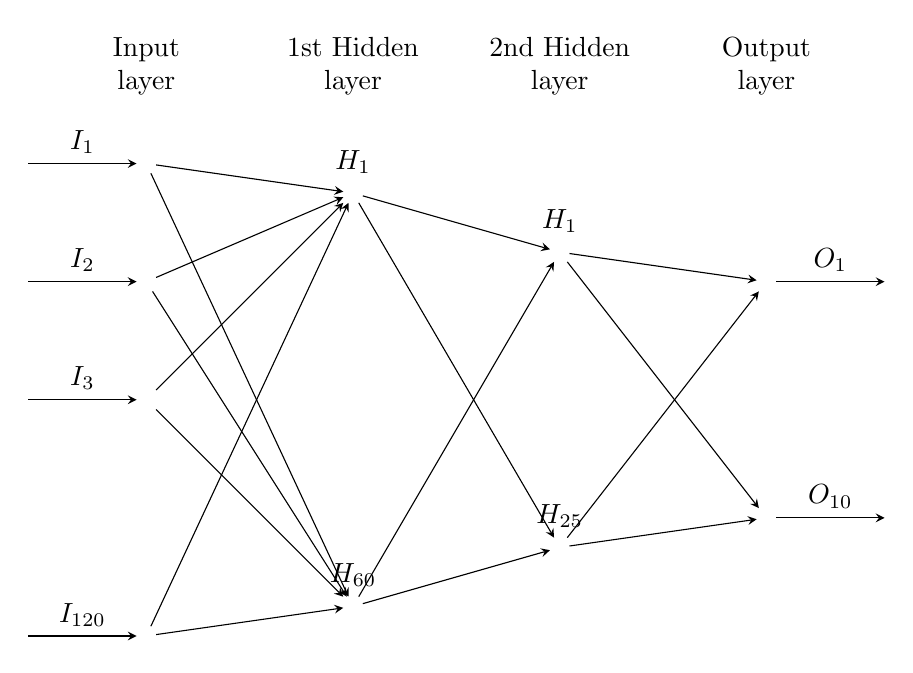
\begin{tikzpicture}[x=1.5cm, y=1.5cm, >=stealth]
        
        % layers
        \foreach \m/\l [count=\y] in {1,2,3,missing,4}
        \node [every neuron/.try, neuron \m/.try] (input-\m) at (0,2.5-\y) {};
        
        \foreach \m [count=\y] in {1,missing,2}
        \node [every neuron/.try, neuron \m/.try ] (hidden-\m) at (1.75,3-\y*1.75) {};
        
        \foreach \m [count=\y] in {1,missing,2}
        \node [every neuron/.try, neuron \m/.try ] (hidden2-\m) at (3.5,2-\y*1.25) {};
        
        \foreach \m [count=\y] in {1,missing,2}
        \node [every neuron/.try, neuron \m/.try ] (output-\m) at (5.25,1.5-\y) {};
        
        %   label
        \foreach \l [count=\i] in {1,2,3,{120}}
        \draw [<-] (input-\i) -- ++(-1,0)
        node [above, midway] {$I_{\l}$};
        
        \foreach \l [count=\i] in {1,60}
        \node [above] at (hidden-\i.north) {$H_{\l}$};
        
        \foreach \l [count=\i] in {1,25}
        \node [above] at (hidden2-\i.north) {$H_{\l}$};
        
        \foreach \l [count=\i] in {1,10}
        \draw [->] (output-\i) -- ++(1,0)
        node [above, midway] {$O_{\l}$};
        
        \foreach \i in {1,...,4}
        \foreach \j in {1,...,2}
        \draw [->] (input-\i) -- (hidden-\j);
        
        \foreach \i in {1,...,2}
        \foreach \j in {1,...,2}
        \draw [->] (hidden-\i) -- (hidden2-\j);
        
        \foreach \i in {1,...,2}
        \foreach \j in {1,...,2}
        \draw [->] (hidden2-\i) -- (output-\j);
        
        \foreach \l [count=\x from 0] in {Input, 1st Hidden, 2nd Hidden, Output}
        \node [align=center, above] at (\x*1.75,2) {\l \\ layer};
        
    \end{tikzpicture}
\end{center}

\paragraph{Activation and loss functions}
The activation function for the input and hidden layers is a \emph{Relu}, 
to prevent \emph{vanishing gradient problem}, 
and the output one uses a \emph{Softmax} to have classification probabilities
among classes.~\cite{relu}\cite{soft}\cite{vanishing}
The loss used is the \emph{Sparse Categorical Crossentropy loss} as it 
is well suited for multiclass classification and, since 
the classes are integers and not one-hot encoded, the sparse version is preferred.~\cite{entropy}

\paragraph{Choosing an optimizer}
When choosing an optimizer for a Neural Network one must take into account the 
cost of reaching a minimum point on the error function.
Although more complex optimizers exists, build to reduce training 
cost on deep networks or to reach a minimum point in less steps, the one choosen 
for this model is a classic Stochastic Gradient Descent optimizer.

Testing some more advanced optimizers shows that convergence is reached faster on the 
networks used in the experiments, but the speed increase is negligible as the model
is quite small.

\subsection{Initial training set results}

Section \vref{feature-extraction} talked about the four different 
training sets obtained from the dataset and, without going into details, 
stated that there was continuous improvement. 
We now give a more detailed look on training performance.

Note that all the random seeds used by Tensorflow were fixed 
to make results reproducible. This step is necessary as many parameters initial 
state are random, for instance, the Neural Network weights.

\paragraph{Class imbalance}
To deal with the minority of some classes, balancing techniques should be 
applied when fitting the model. One of the possible approaches, and the one followed
here, is to assign class weights. 

The main idea is to penalize errors made on not well represented classes, to account 
for their minority. To compute class weights, the \emph{compute class weights} function
from sklearn was used.~\cite{classweight}

The following are the computed quantities for the dataset classes:
\begin{center}
    \begin{tabular}{ |l|c|c| } 
        \hline
        Class name & Number of samples & Class weight \\
        \hline
        air conditioner & 500 & 0.8998 \\
        car horn & 208 & 2.1629 \\
        children playing & 500 & 0.8998 \\
        dog bark & 500 & 0.8998 \\
        drilling & 500 & 0.8998 \\
        engine idling & 517 & 0.8702 \\
        gun shot & 190 & 2.3678 \\
        jackhammer & 548 & 0.8209 \\
        siren & 536 & 0.8393 \\
        street music & 500 & 0.8998 \\
        \hline
    \end{tabular}
\end{center}
As expected, the less numerous classes have higher class weight than the rest. 
In particular, the misclassification of a car horn class sample
counts almost 2.5 times more than an air conditioner one.

\paragraph{Stratified cross-validation}
To estimate performance on the training set stratified cross-validation with 
five folds was used. Basically the dataset is divided into five parts 
and a model is repeatly trained on four and tested on one, all while considering class 
distribution, indeed, the original distribution of the classes is maintained 
in the splits.~\cite{stratified}

The stratified approach is required as there is class imbalance on the training set.
In fact, applying a classical cross-validation could show misleading results, 
for instance when the minority classes are more present 
in the test fold rather than the training ones; in such cases the loss would be 
higher.

The mean accuracy on the test folds gives a hint about the model performance.
For this step the \emph{Stratified KFold} class from scikit learn was used.~\cite{cross-scikit}

\paragraph{Results}
For each presented training set, a model was defined 
with the structure presented at the beginning of this Section, 
and these are the results:

\begin{center}
    \begin{tabular}{ |l|r|r| } 
        \hline
        Training set & Mean accuracy & St. deviation \\
        \hline
        132 features unscaled &  0.1138 & 0.0039 \\
        132 features scaled &  0.5743 & 0.0324 \\
        144 features scaled &  0.6079 & 0.0486 \\
        120 features reduced with PCA &  0.6143 & 0.0481 \\
        \hline
    \end{tabular}
\end{center}

There is a great improvement after scaling the training set, after 
that small refinements were made.
As accuracy is the best on the last dataset, this was the one selected to 
perform the Hyperparameter tuning.

\subsection{Hyperparameter tuning}

Choosing the training set with PCA applied led to the best results 
with stratified cross-validation. Although the model was reasonable, 
it can not be the final one, as many parameters are left on their default value, 
for instance, learning rate and momentum of the optimizer are untouched. 

The main goal now is to experiments with ranges of model parameters 
to find a better one.

\paragraph{Grid and Random search comparison}
Two of the most commonly used strategies in Hyperparameter optimization
are \emph{Grid} and \emph{Random Search}~\cite{random-grid}. 

In both cases we define ranges of parameters to test different combinations, 
for instance, fixed the number of neurons, one could try to find the best 
combination of learning rate and momentum that optimize accuracy on the training set.

While similar, the two methodologies differs in the amount of exploration they do.
The Grid search try all the possible combinations of parameters, while the 
Random approach fixes a number of iterations and picks an arbitrary combination each time. 

Obviously the first one is more computationally expensive than the second, if 
we fix a small amount of possible iterations, but in theory it finds a better result
than going the random route. 
Nonetheless the Grid Search can led to over-fitting, and in practice Random 
Search in preferred.

\paragraph{Random search}
We now run a Random Search with various model parameters 
to optimize the initial model.
Note that class weights are still considered and the models are evaluated
again with a stratified cross-validation.
The optimizer used is the Stochastic Gradient Descent.
The considered ranges for parameters for this run are: 
\begin{enumerate}
    \item \emph{Neurons}: first and last layers stay the same, while 
    the two hidden layers are tested with a number of neurons respectively 
    equals to: 
    $$60 + 2i\;\;\text{and}\;\;25 + 2j,\;\;\text{with}\;\; i, j \in \{-2,-1,0,1,2\}$$
    \item \emph{Learning rate}: $0.001, 0.01, 0.1, 0.5$;
    \item \emph{Momentum}: $0.0, 0.01, 0.1, 1$.
\end{enumerate}

The models are fitted with 100 \emph{epochs} and \emph{batch size} equals to 32.
An early stopped is used on the training to stop it when no progress is made with 
respect to the last epoch results.
The total possible models are 400, but the search was performed with 100 iterations
in total.

\paragraph{Final model}
The best model found is the following: 
\begin{itemize}
    \item \emph{Neurons}: 120 for input, 62 for the first hidden layer, 27 for the second, and 10 for output; 
    \item \emph{Momentum}: 0.0;
    \item \emph{Learning rate}: 0.1.
\end{itemize}
Comparing the initial model with the one found now, a small improvement 
can be seen in accuracy despite a worse standard deviation:
\begin{center}
    \begin{tabular}{ |l|r|r| } 
        \hline
        Model & Mean accuracy & St. deviation \\
        \hline
        Initial model & 0.6143 & 0.0481\\
        Random search result & 0.6297 & 0.0530 \\
        \hline
    \end{tabular}
\end{center}
This model is the one chosen to evaluate performance on the test sets.
\newpage